\chapter{Testy}  \label{ch:CHAPTER_3}
\thispagestyle{chapterBeginStyle}


\section{Informacje wstępne}
Zbiór danych na których zostały przeprowadzone testy znajduje się w katalogu \verb|Tests/input|. Każdy z dziesięciu plików, których nazwy trzymają się konwencji: test$<$numer\_testu$>$.txt, jest zgodny z formatem opisanym w sekcji \ref{format_danych}, gdzie $<$numer\_testu$>$ to liczba naturalna ze zbioru $\{0, ..., 9\}$.

Do pomiaru czasu wykonania zostało wykorzystane linuksowe polecenie \textbf{time} - brana pod uwagę była tylko ilość czasu procesora spędzonego w kodzie w trybie użytkownika. Pominięty został czas spędzony w jądrze systemu - czytanie wejścia, alokacje pamięci.

Za automatyzację uruchamiania programu na poszczególnych plikach i algorytmach odpowiada skrypt napisany w języku powłoki bash - plik \verb|Tests/run_tests.sh|. Iteruje on po plikach z katalogu w którym znajduja się dane testowe, po algorytmach, wyznacza nazwy plików według określonego schematu i wywołuje komendę: \\
\verb|{ time $EXEC_FILE -f $infile -o $resultfilename -a $algo > $solver_log ;} 2> $time_filename|, 

\begin{itemize}
	\item \$EXEC\_FILE - ścieżka do skompilowanego programu
	\item \$infile - plik z danymi wejściowymi: \\
	\verb|Tests/input/test<numer_testu>.txt|
	\item \$resultfilename - ścieżka do pliku z rozwiązaniem: \\ \verb|Tests/output/test<numer_testu>_<algorytm>_res.txt| (patrz rysunek \ref{output_example})
	\item \$algo - algorytm (APPROX, MIP, SM)
	\item \$solver\_log - ścieżka do pliku w którym zostanie zapisane standardowe wyjście programu, a na które drukuje bibliotek GLPK podczas optymalizacji
	\item \$time\_filename - ścieżka do pliku z rezulatatem polecenia \textbf{time}
\end{itemize}

Wykresy i tabele wyegenrowane zostały za pomocą skryptu pythonowego: \\ \verb|Tests/generate_plots.py|.

Oznaczenia:
\begin{itemize}
	\item APPROX - program używał algorytmu aproksymacyjnego
	\item MIP - program używał solvera MIP (branch and cut)
	\item SM - program używał solver simpleksowego i zaokrąglał wyniki algorytmem aproksymacyjnym
\end{itemize}

Platforma testowa to komputer stacjonarny z czterordzeniowym procesorem Intel Core i5-3570K, 16GB pamięci RAM DDR3 CL9.

Warto dodać, że test numer dwa pochodzi od EURO Special Interest Group on Cutting and Packings. Dane testowe przez nich dostarczone można znaleźć pod tym linkiem:
\href{https://www.euro-online.org/websites/esicup/data-sets/}{ESICUP dataset}.
Konkretnie jest to pozycja \textit{The 28 VERY hard BPP instances of J. Schoenfield (with m from 140 to 200). Test results with an LP-based approach in (Data sets: hard28)} - próba o nazwie \textit{'BPP    14'}. Zawiera on podobny format danych opisanych wcześniej z tą różnicą, że długośc belki i liczba elementów są zamienione wierszami. Jednakże testowany w tej pracy przykład rozpatruje najmniejszy element długości 40 - stąd liczba typów 126 zamiast pierwotnych 136. Spowodowane było to problemem z wykorzystaniem całej dostępnej pamięci operacyjnej platformy testowej dla drugiej wartości. Owe dane testowe łamią też w pewnym sensie koncepcję przyjęcia za liczbę typów stałej. Największa liczba elementów danego typu jaka występuje to 2, zazwyczaj wynosi ona jeden, więc pomimo liczby typów wynoszącej 126, wszystkich elementów jest 148. Same instancje problemów zostały określone jako \textit{bardzo trudne}.



\begin{table}[H] 
	\begin{center}
		\begin{tabular}{|p{3cm}|p{3cm}|p{3cm}|p{3cm}|p{3cm}| } \hline
			Numer testu & Długość belki & Liczba typów elementów & Liczba wszystkich elementów ($n$) & Liczba wygenerowanych konfiguracji\\ 
			\hline
			0 & 5600 & 13 & 219 & 213\\ 
			1 & 1200 & 4 & 343 & 3563\\ 
			2 & 1000 & 126 & 148 & 7682204\\ 
			3 & 600 & 10 & 225 & 636\\ 
			4 & 6000 & 12 & 178 & 6506312\\ 
			5 & 4500 & 18 & 190 & 1506800\\ 
			6 & 7300 & 12 & 130 & 1632979\\ 
			7 & 120 & 10 & 227 & 614\\ 
			8 & 3000 & 15 & 187 & 824526\\ 
			9 & 1000 & 12 & 394 & 1459890\\ 
			
			\hline
		\end{tabular}
		\caption{Podstawowe dadne dotyczące poszczególnych testów.}
	\end{center}
\end{table}


\section{Wyniki}

Dla każdego testu solver był w stanie znaleźć rozwiązanie i zwrócił komunikaty:
\begin{itemize}
	\item ``OPTIMAL LP SOLUTION FOUND`` dla metody simpleksowej
	\item ``INTEGER OPTIMAL SOLUTION FOUND`` dla metody MIP
\end{itemize}

\subsection{Liczba belek}

%\iffalse

\begin{table}[H] 
	\begin{center}
	\begin{tabular}{|p{3cm}|p{3cm}|p{3cm}|p{3cm}|p{3cm}| } 
		\hline
			Numer testu & APPROX & SM & MIP & Dolna granica\\ 
			\hline
			0 & 82 & 73 & 73 & 73\\ 
			1 & 13 & 13 & 13 & 13\\ 
			2 & 62 & 61 & 61 & 61\\ 
			3 & 91 & 92 & 91 & 84\\ 
			4 & 11 & 11 & 10 & 10\\ 
			5 & 37 & 37 & 37 & 37\\ 
			6 & 19 & 19 & 19 & 19\\ 
			7 & 61 & 61 & 60 & 60\\ 
			8 & 23 & 23 & 23 & 23\\ 
			9 & 51 & 51 & 51 & 51\\ 
			\hline
		\end{tabular}
			\caption{Liczba belek dla poszczególnych algorytmów w zależności od numeru testu.}
	\end{center}
\end{table}

\begin{figure}[H]
	\begin{center}
	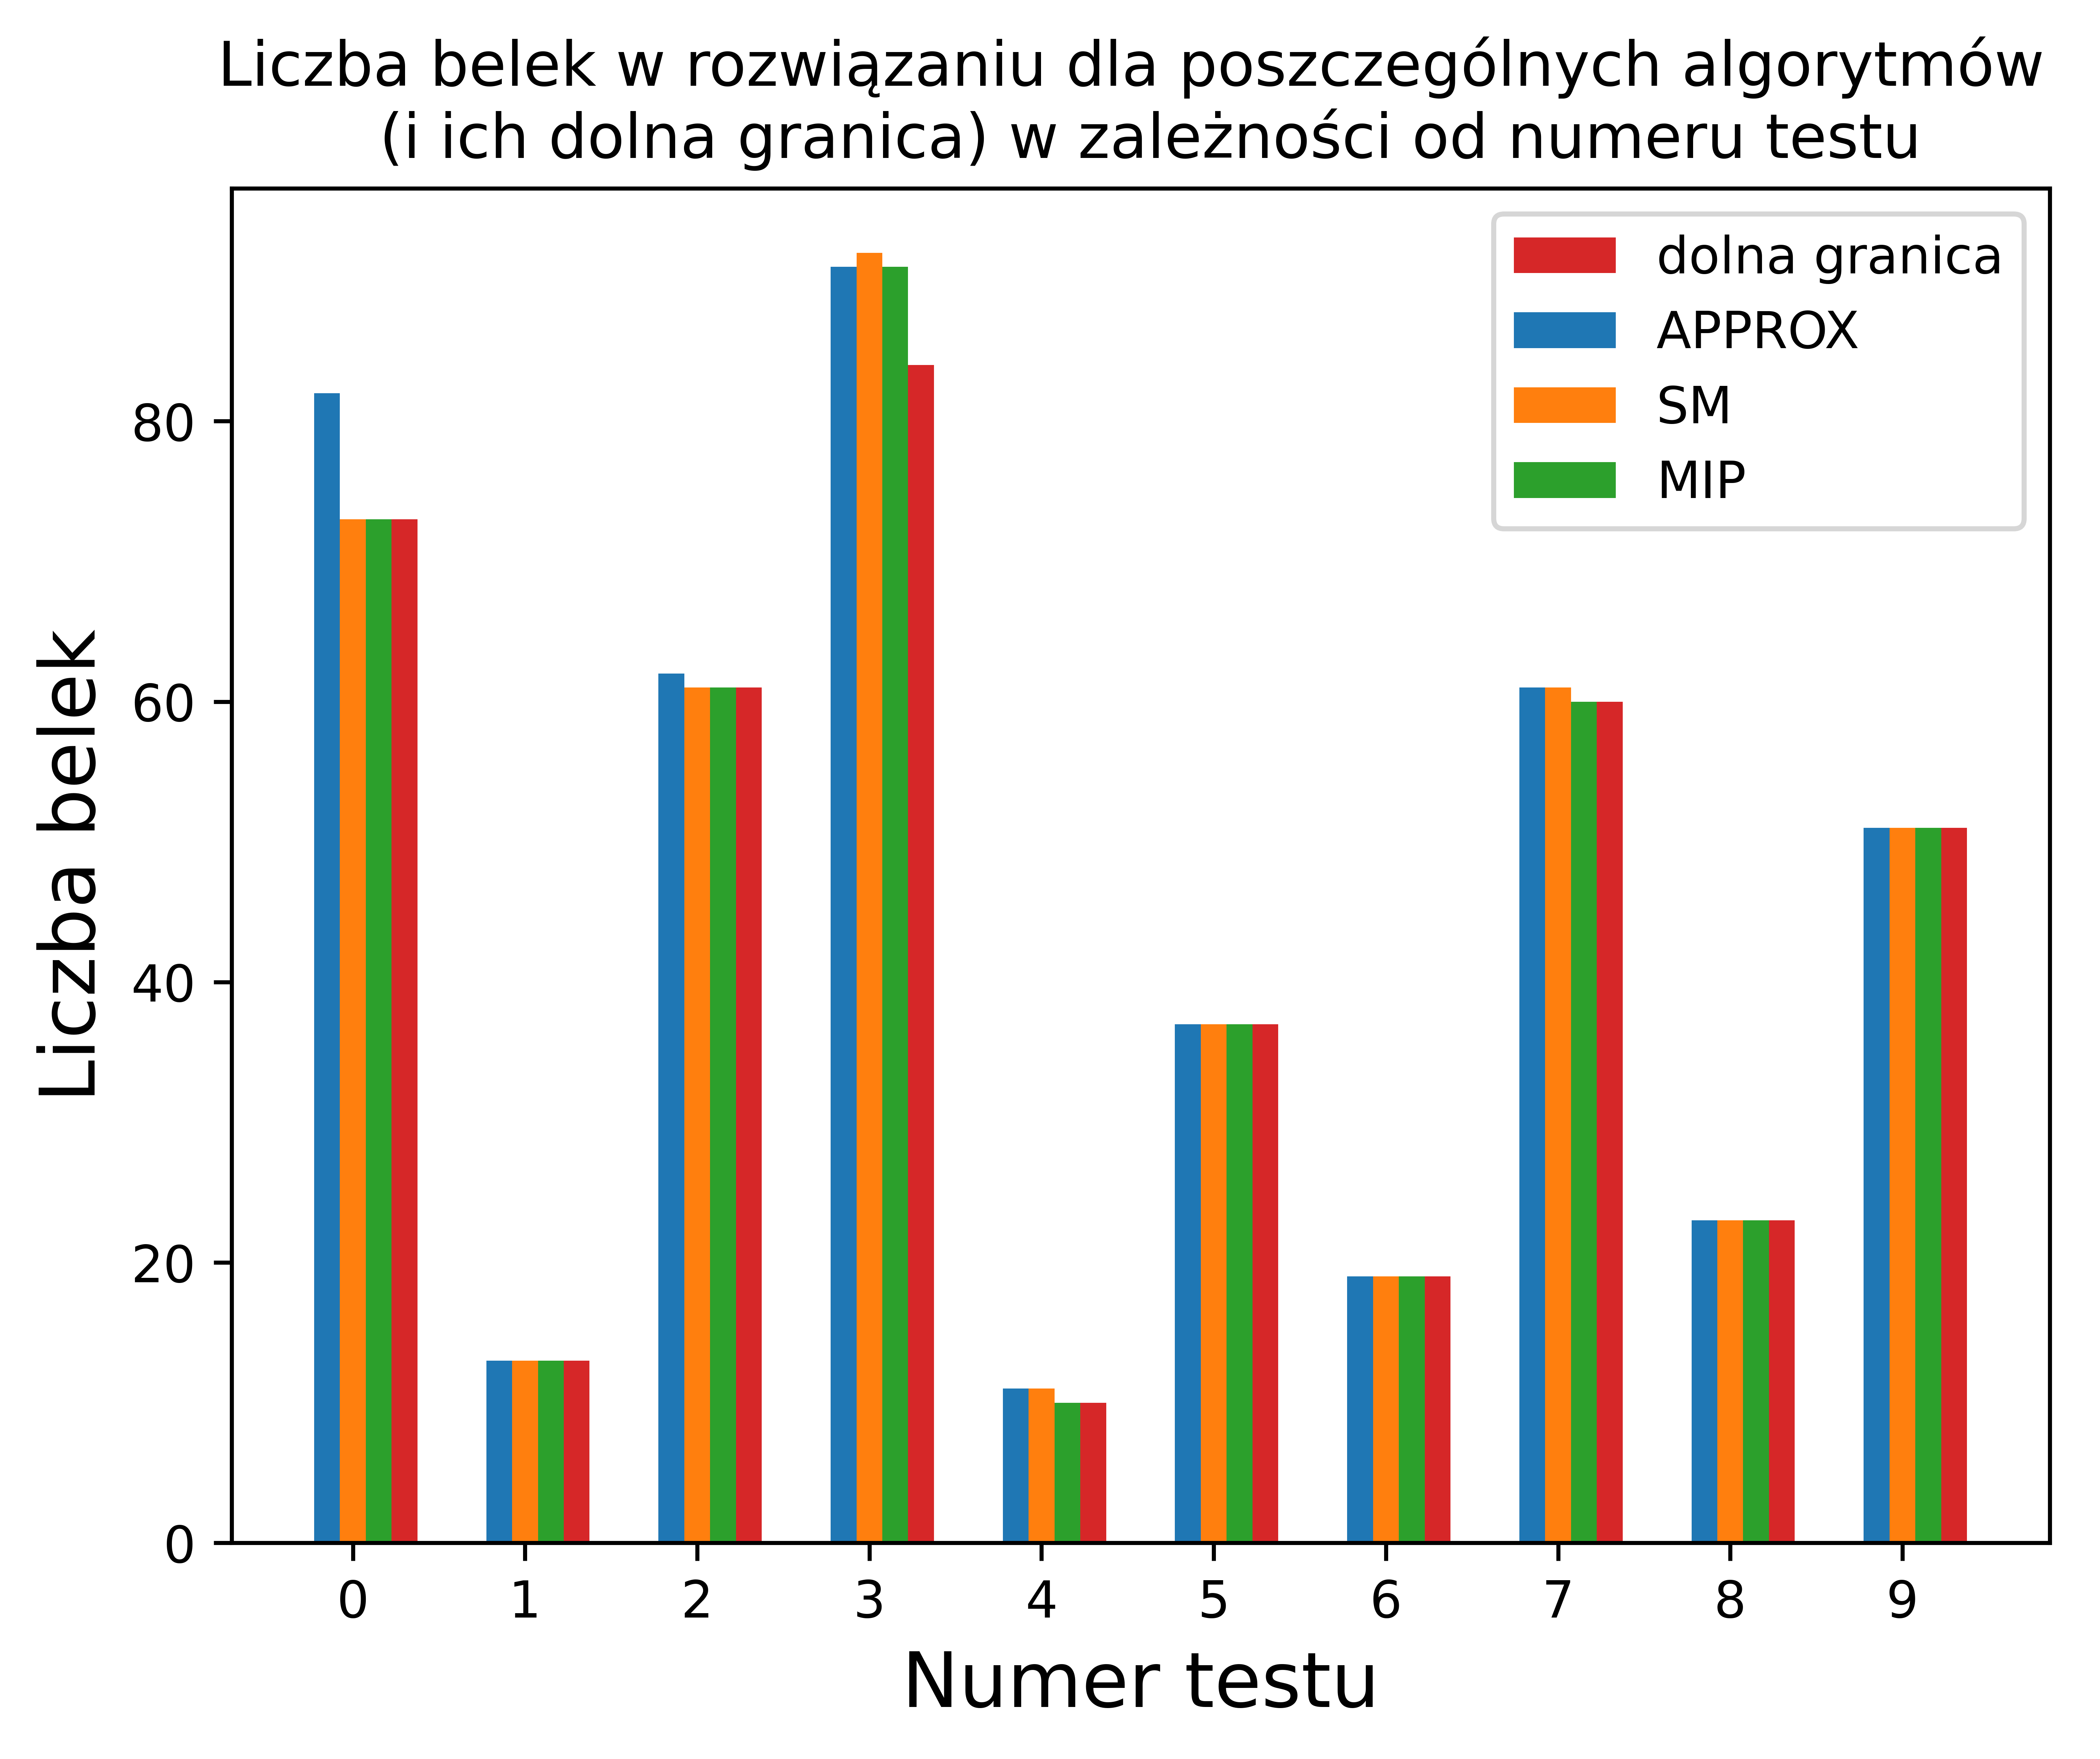
\includegraphics[width=12cm]{plots/res}
	\caption{Wykres przedstawiający liczbę belek (i ich dolną granicę) w rozwiązaniu dla poszczególnych algorytmów w zależności od numeru testu.}
	\end{center}
\end{figure}

\begin{figure}[H]
	\begin{center}
		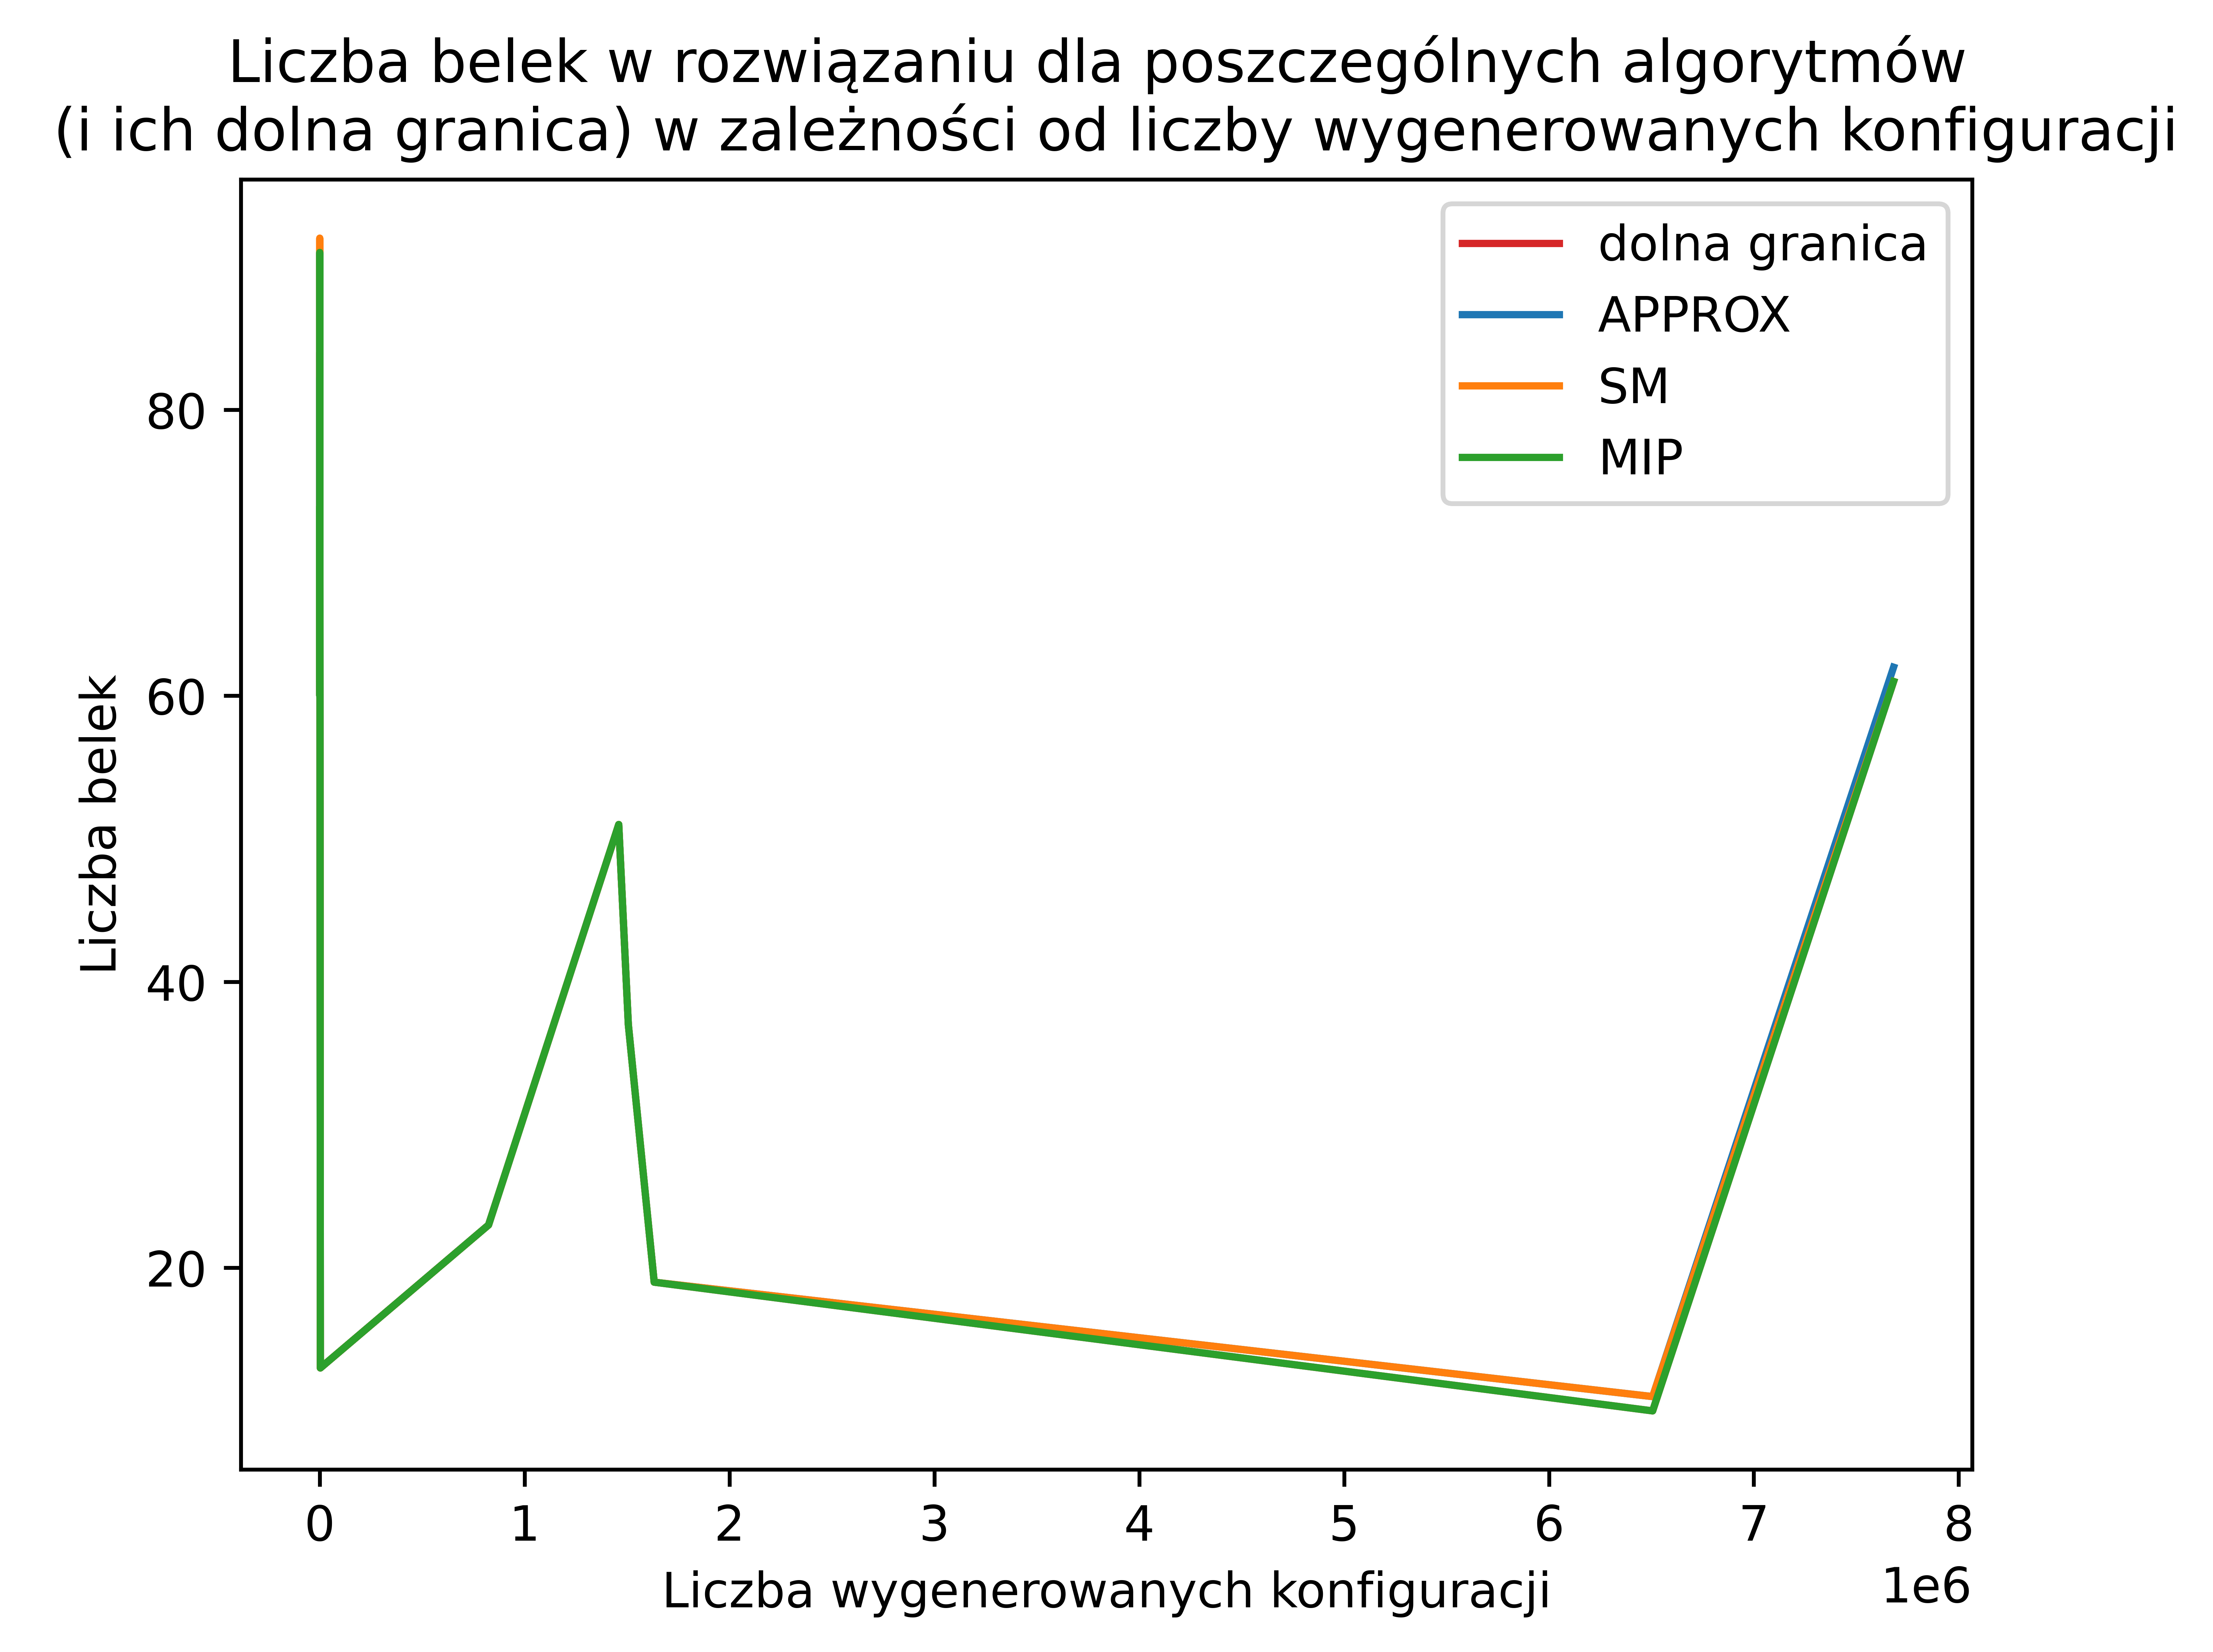
\includegraphics[width=12cm]{plots/res_configs}
		\caption{Wykres przedstawiający liczbę belek (i ich dolną granicę) w rozwiązaniu dla poszczególnych algorytmów w zależności od liczby wygenerowanych konfiguracji.}
	\end{center}
\end{figure}

\subsection{Czas wykonania}


\begin{table}[H] 
	\begin{center}
		\begin{tabular}{|p{3cm}|p{3cm}|p{3cm}|p{3cm}| } \hline
			Numer testu & APPROX & SM & MIP\\ 
			\hline
			0 & 0.001 & 0.002 & 0.006\\ 
			1 & 0.001 & 0.000 & 0.050\\ 
			2 & 0.002 & 178.151 & 9849.150\\ 
			3 & 0.001 & 0.000 & 0.003\\ 
			4 & 0.001 & 6.527 & 1343.093\\ 
			5 & 0.000 & 4.271 & 1164.734\\ 
			6 & 0.001 & 3.837 & 742.420\\ 
			7 & 0.000 & 0.002 & 0.017\\ 
			8 & 0.001 & 1.533 & 417.277\\ 
			9 & 0.001 & 1.804 & 84.618\\ 
			\hline
		\end{tabular}
		\caption{Czas wykonania progamu (w sekundach) dla poszczególnych algorytmów i testów.}
	\end{center}
\end{table}

\begin{figure}[H]
	\begin{center}
		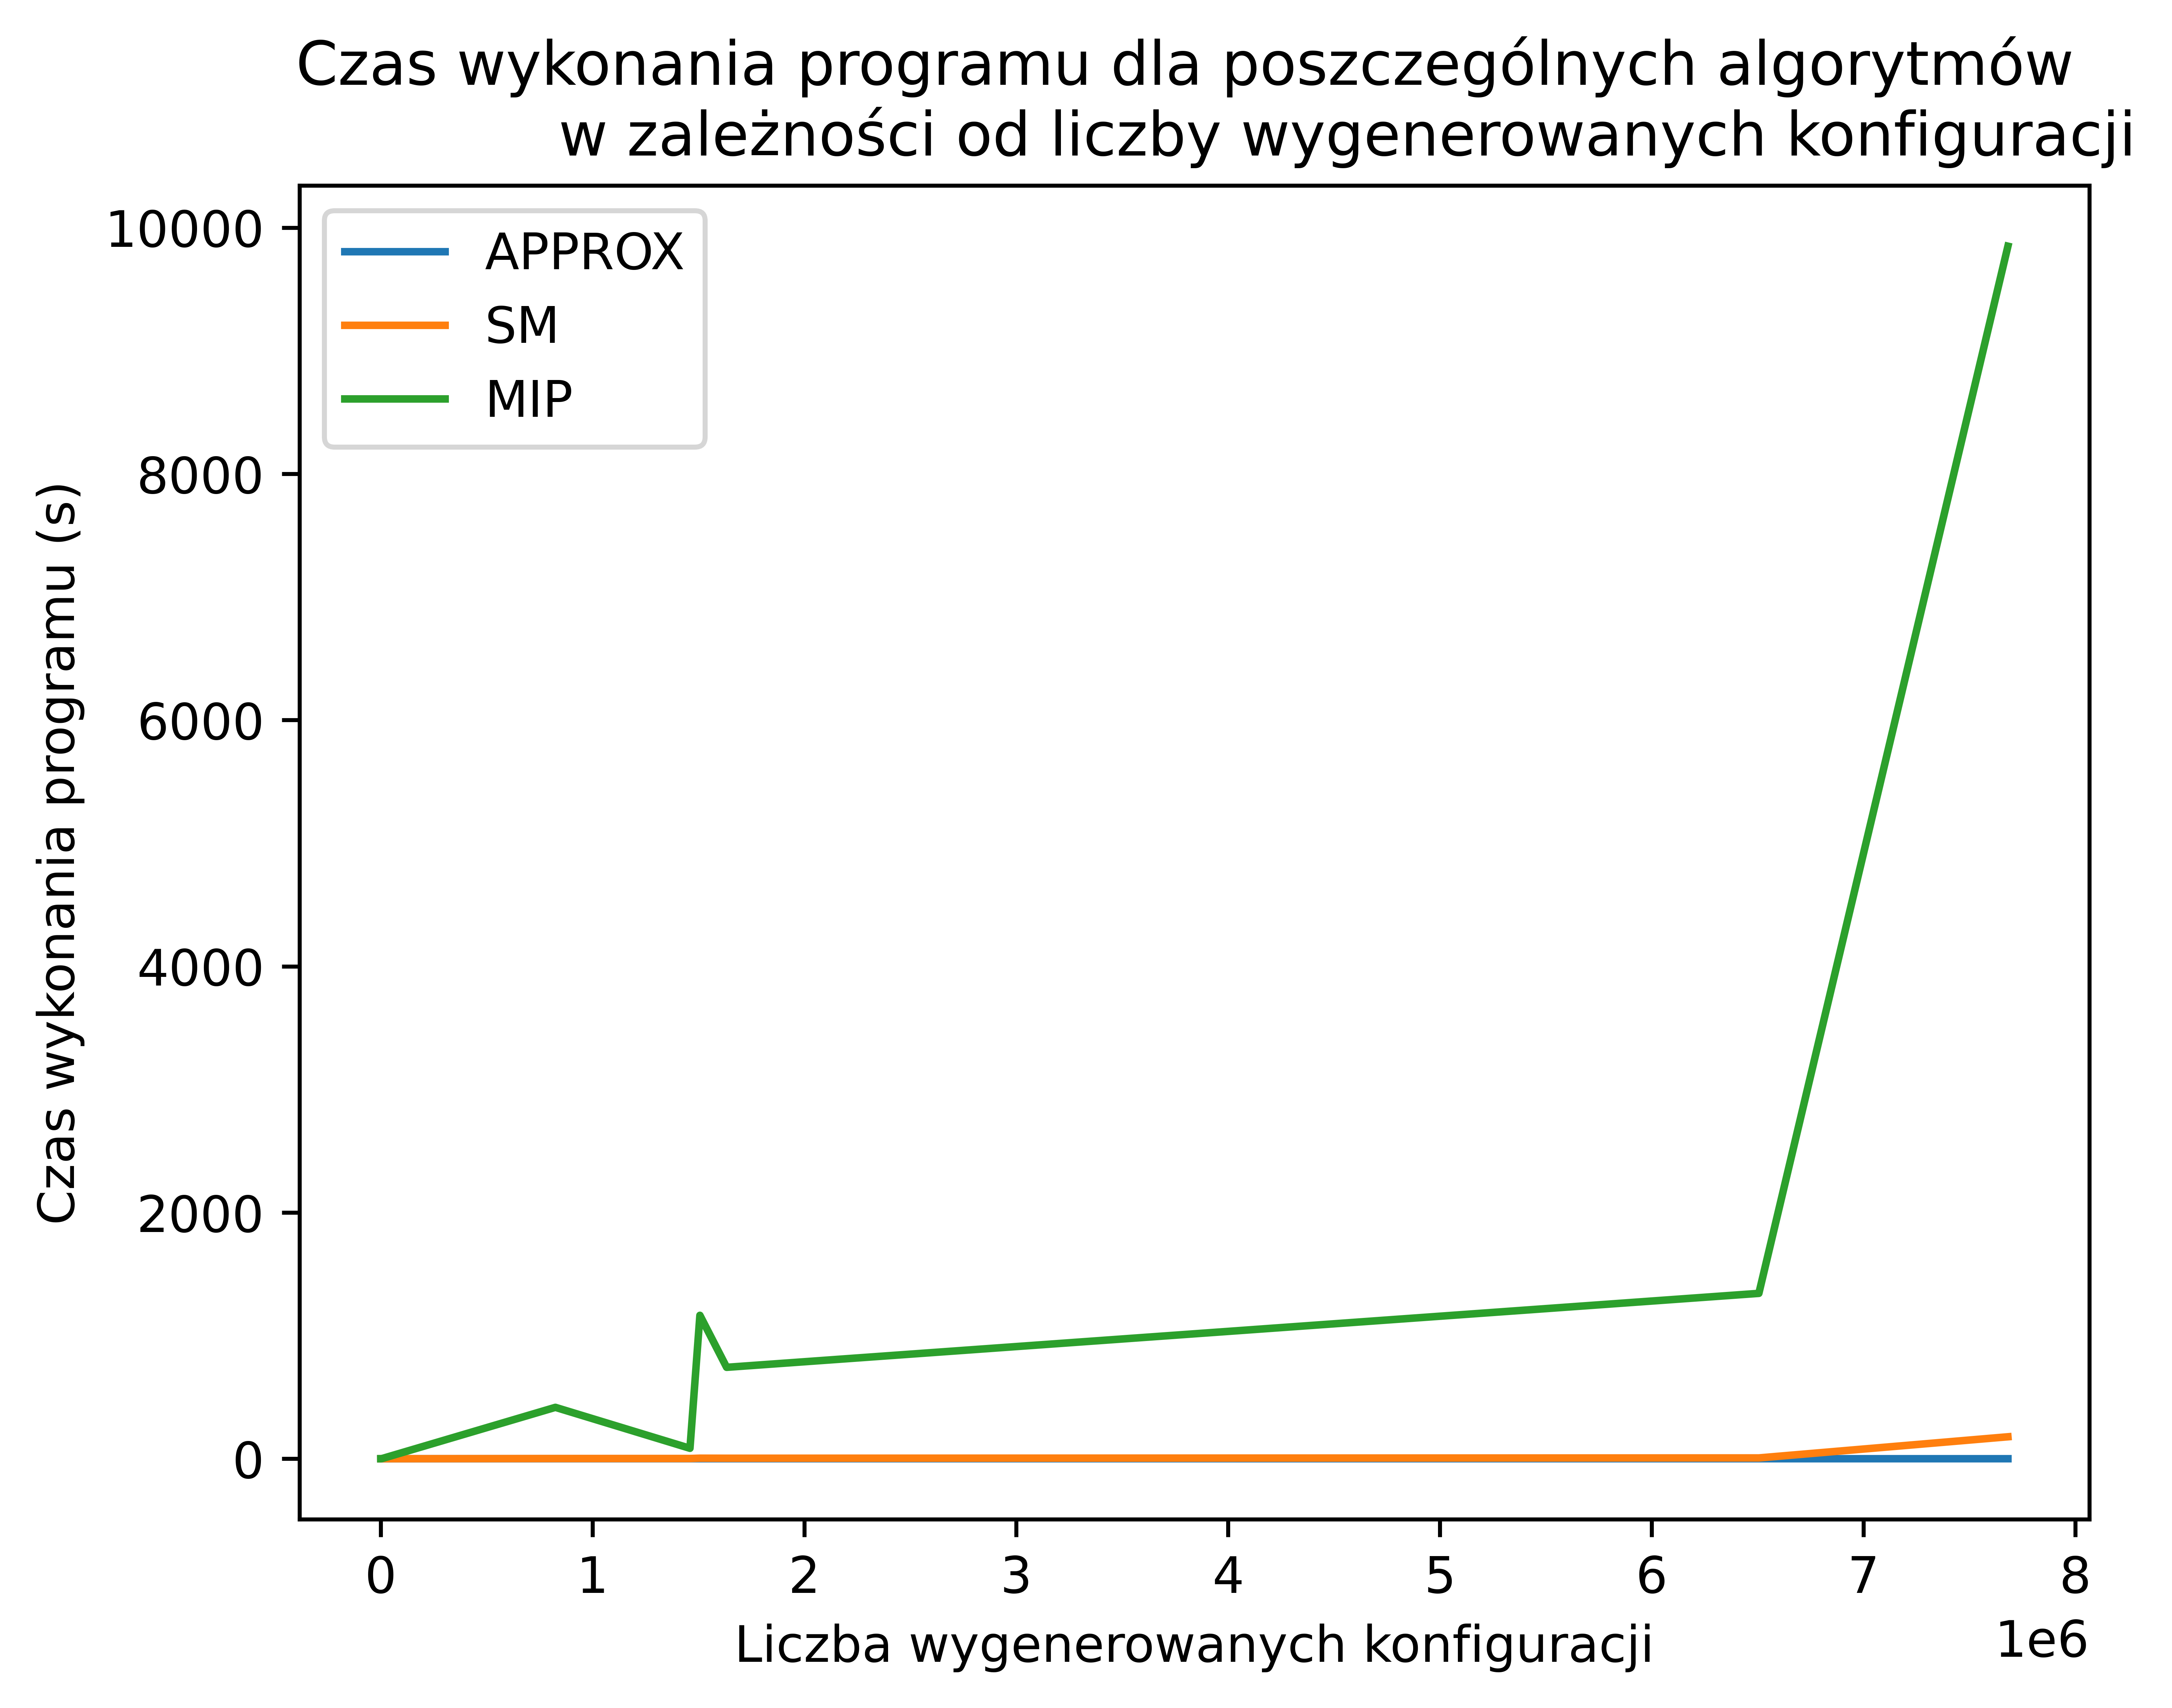
\includegraphics[width=12cm]{plots/time_configs}
		\caption{Wykres przedstawiający czas wykonania programu dla poszczególnych algorytmów w zależności od liczby wygenerowanych konfiguracji.}
	\end{center}
\end{figure}
%\fi

\newpage
\section{Obserwacje}

Z powyższych danych można zauważyć, że
\begin{itemize}
	\item otrzymane rozwiązania są często blisko dolnej granicy:
	\begin{itemize}
		\item jej równe w pięciu, większe o jeden w trzech przypadkach dla APPROX \\
		Tylko w teście numer zero różnica ta wynosiła dziewięć belek na niekorzyść tej metody, co daje w przybliżeniu 112,32 procent kosztu rozwiązania optymalnego. Owa wartość mieści się w absolutnym współczynniku aproksymacji tego problemu: $3/2$, jednak wykracza poza średni wynoszący dla algorytmu FFD $11/9$.
		\item jej równe w siedmiu, większe o jeden w trzech przypadkach dla SM
		\item jej równe w dziewięciu przypadkach dla MIP
	\end{itemize}
	\item Algorytmy posiadają bardzo zróżnicowany czas działania.
	Program używający algolrytmu aproksymacyjnego nie przekroczył nigdy dwóch milisekund, a najszęsciej nawet jednej - stąd wartość zero w tabelach i wykresach. Natomiast MIP potrafił działać nawet prawie trzy godziny (test drugi - 9849.150s) zanim znalazł optymalne rozwiązanie. 
	\item Znaczący wpływ na liczbę możliwych konfiguracji ma duża liczba małych elementów.
	
\end{itemize}

\section{Wnioski}

\begin{itemize}
	\item Dla wielu instancji problemu cięcia belek może sie okazać, że rozwiązanie obliczone przy pomocy algorytmy aproksymacyjnego FFD będzie często bliskie rozwiązania optymalnego.
	\item W przypadku optymalizacji dyskretnej dużo czasu zajmuje znalezienie rozwiązania optymalnego pod kątem całkowitoliczbowym, w kontraście do szybkiego znajdowania optymalnego rozwiązania problemu pochodnego (poddanego relaksacji) algorytmem simpleks.
	\item Potwierdza się informacja dotycząca metody branch-and-cut zawarta w dokumentacji: \textit{GLPK branch-and-cut solver is not perfect, so it is unable to solve hard or very large scale MIP instances for a reasonable time.} Gdyby zwiększyć liczbę potrzebnych małych elementów do dwudziestu dla każdego rodzaju, program działałby dłużej niż najdłuższy zaprezentowany test (powyżej trzech godzin).
	\item Generowanie wszystkich możliwych konfiguracji i decydowanie o ich wyborze po fakcie ich wygenerowania nie sprawdzi się w przypadku maszyn z małą ilościa pamięci operacyjnej.
\end{itemize}






